Now, let us consider the wave equation in 3+1 dimensions with spherical symmetry:
%
\begin{equation}
    \Box \psi \equiv - \partial_T^2 \psi + \frac{1}{R^2} \partial_R\left( R^2 \partial_R \psi\right) = 0 \;.
\end{equation}

Since $\psi$ is a solution to this equation, it will decay at a rate of $1/R$, which is a problem because we want to know how our field behaves at $\mathscr{I}$. Thus, we need to renormalize this field so it does not vanish at infinity. With this in mind, let us define a new field $\Psi$ such that
%
\begin{equation}
    \Psi \equiv \chi \, \psi \; ,
\end{equation}
%
where we will take $\chi = \sqrt{1+R^2}$.

Applying that transformation to the equation, it becomes
%
\begin{equation}
    \partial_T^2 \Psi = \partial_R^2\Psi + \frac{2}{R(R^2+1)} \partial_R\Psi - \frac{3}{(R^2+1)^2} \Psi \;,
\end{equation}
%
to which we can apply a first-order reduction, obtaining
%
\begin{equation}
    \left\{ \begin{array}{l} 
        \partial_T \Psi = - \Pi \\ 
        \partial_T \Phi = - \partial_R \Pi + \gamma_2 \partial_R \Psi - \gamma_2\Phi\\
        \partial_T \Pi = - \partial_R \Phi - \frac{2}{R(R^2+1)}\Phi + \frac{3}{(R^2+1)^2} \Psi
    \end{array} \right. \; .
\end{equation}

Doing a coordinate change from inertial Minkowski coordinates to hyperboloidal coordinates and setting $\gamma_2 = 0$ as we did previously, we get
%
\begin{equation}
    \left\{ \begin{array}{l} 
        \partial_T \Psi = - \Pi \\ 
        \partial_T \Phi = \mathcal{B}\left((r^2 + \Omega^2)^2 \left(H' \partial_r \Phi + \partial_r\Pi\right) + H' L \Omega \left( 2r\Phi - 3 \Omega \Psi + 2 r^{-1} \Omega^2 \Phi\right)\right)\\
        \partial_T \Pi = \mathcal{B}\left((r^2 + \Omega^2)^2 \left(\partial_r \Phi + H' \partial_r\Pi\right) + L \Omega \left( 2r\Phi - 3 \Omega \Psi + 2 r^{-1} \Omega^2 \Phi\right)\right)
    \end{array} \right. \; ,
\end{equation}
where we defined $\mathcal{B}= \frac{\Omega^2}{L(H'^{\,2}-1)(r^2 + \Omega^2)^2}$. 

We can see that in our evolution equations for $\Phi$ and $\Pi$, there are formally singular terms we can remove by applying the Evans method. For that, we rewrite those evolution equations, obtaining
%
\begin{equation}
    \left\{ \begin{array}{l} 
        \partial_T \Psi = - \Pi \\ 
        \partial_T \Phi = \mathcal{B}\left((r^2 + \Omega^2)^2 \left(H' \partial_r \Phi + \partial_r\Pi\right) + H' L \Omega \left( 2r\Phi - 3 \Omega \Psi - \Omega^2 \partial_r \Phi\right) + H' L\Omega^3\left( \partial_r \Phi + 2 r^{-1}\Phi\right) \right)\\
        \partial_T \Pi = \mathcal{B}\left((r^2 + \Omega^2)^2 \left(\partial_r \Phi + H' \partial_r\Pi\right) + L \Omega \left( 2r\Phi - 3 \Omega \Psi - \Omega^2 \partial_r\Phi \right) + L \Omega^3\left( \partial_r \Phi + 2 r^{-1}\Phi \right) \right)
    \end{array} \right. \; ,
\end{equation}
%
where we can directly apply the Evans method to the last terms in parenthesis.

Imposing the parity of each field at the origin and doing extrapolation at $\mathscr{I}$ (instead of truncation error matching that we used before) as our boundary conditions and using the initial data
%
\begin{equation}
    \begin{array}{c c c c}
        \psi(0,r) = A \, e^{-C \, r^2/2} \; , & \Phi(0,r) = - A \,C \, r \, \frac{\Omega^2(r)}{L(r)} \, e^{-C \, r^2/2} & \text{and} & \Pi(0,r) = 0
    \end{array} \; ,
    \label{eq:spherical_compact_wave_equation-2nd_order_initial_conditions}
\end{equation}
with $A = 1$ and $C = 100$, we obtain the evolution represented in figure \ref{fig:spherical_compact_wave_equation-2nd_order}.

\begin{figure}[h]
    \centering
    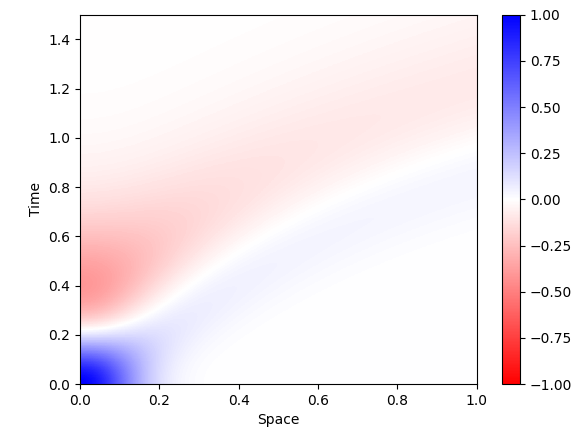
\includegraphics[width=0.5\textwidth]{Images/Wave_Equation_3+1_Spherical-Solution.png}
    \caption{Evolution of the wave equation in 3+1 dimensions with spherical symmetry using hyperboloidal coordinates with the initial conditions given in equation \eqref{eq:spherical_compact_wave_equation-2nd_order_initial_conditions}, with $A = 1$ and $C = 100$.}
    \label{fig:spherical_compact_wave_equation-2nd_order}
\end{figure}

Similarly to the previous case, we obtain a clean second-order convergence during the whole evolution, shown in the left of figure \ref{fig:spherical_compact_wave_equation-2nd_order-convergence} for $\psi$, and an excellent pointwise convergence at $\mathscr{I}$, as seen in the right of figure \ref{fig:spherical_compact_wave_equation-2nd_order-convergence}. Even though these results are already outstanding, they could be further improved by using truncation error matching at the outer boundary instead of extrapolation.

\begin{figure}[h]
    \centering
    \begin{subfigure}[b]{0.45\textwidth}
        \centering
        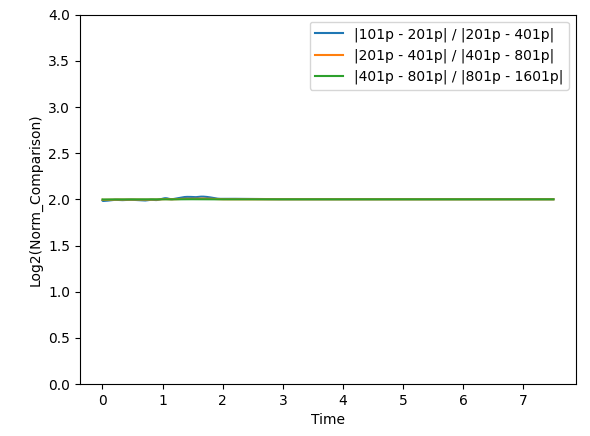
\includegraphics[width=\textwidth]{Images/Wave_Equation_3+1_Spherical-Norm.png}
    \end{subfigure}
    \hfill
    \begin{subfigure}[b]{0.45\textwidth}
        \centering
        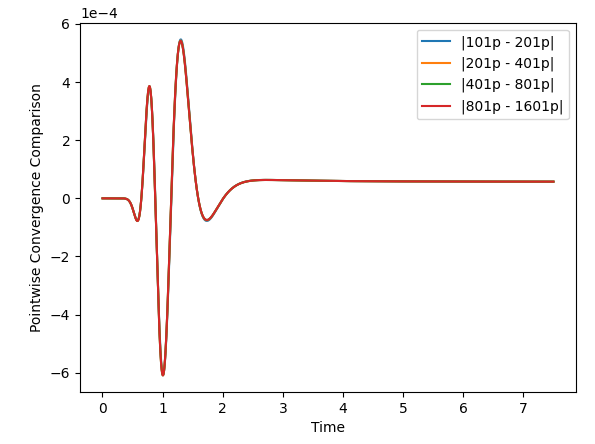
\includegraphics[width=\textwidth]{Images/Wave_Equation_3+1_Spherical-Pointwise.png}
    \end{subfigure}
    \caption{Convergence tests for the evolution of the wave equation in 3+1 dimensions with spherical symmetry using hyperboloidal coordinates, provided the initial conditions given in equation \eqref{eq:spherical_compact_wave_equation-2nd_order_initial_conditions}, with $A = 1$ and $C = 100$.. On the left, we have the $L^2$ norm convergence, and on the right, we have the pointwise convergence at $\mathscr{I}$.}
    \label{fig:spherical_compact_wave_equation-2nd_order-convergence}
\end{figure}